
%% bare_conf.tex
%% V1.3
%% 2007/01/11
%% by Michael Shell
%% See:
%% http://www.michaelshell.org/
%% for current contact information.
%%
%% This is a skeleton file demonstrating the use of IEEEtran.cls
%% (requires IEEEtran.cls version 1.7 or later) with an IEEE conference paper.
%%
%% Support sites:
%% http://www.michaelshell.org/tex/ieeetran/
%% http://www.ctan.org/tex-archive/macros/latex/contrib/IEEEtran/
%% and
%% http://www.ieee.org/

%%*************************************************************************
%% Legal Notice:
%% This code is offered as-is without any warranty either expressed or
%% implied; without even the implied warranty of MERCHANTABILITY or
%% FITNESS FOR A PARTICULAR PURPOSE! 
%% User assumes all risk.
%% In no event shall IEEE or any contributor to this code be liable for
%% any damages or losses, including, but not limited to, incidental,
%% consequential, or any other damages, resulting from the use or misuse
%% of any information contained here.
%%
%% All comments are the opinions of their respective authors and are not
%% necessarily endorsed by the IEEE.
%%
%% This work is distributed under the LaTeX Project Public License (LPPL)
%% ( http://www.latex-project.org/ ) version 1.3, and may be freely used,
%% distributed and modified. A copy of the LPPL, version 1.3, is included
%% in the base LaTeX documentation of all distributions of LaTeX released
%% 2003/12/01 or later.
%% Retain all contribution notices and credits.
%% ** Modified files should be clearly indicated as such, including  **
%% ** renaming them and changing author support contact information. **
%%
%% File list of work: IEEEtran.cls, IEEEtran_HOWTO.pdf, bare_adv.tex,
%%                    bare_conf.tex, bare_jrnl.tex, bare_jrnl_compsoc.tex
%%*************************************************************************

% *** Authors should verify (and, if needed, correct) their LaTeX system  ***
% *** with the testflow diagnostic prior to trusting their LaTeX platform ***
% *** with production work. IEEE's font choices can trigger bugs that do  ***
% *** not appear when using other class files.                            ***
% The testflow support page is at:
% http://www.michaelshell.org/tex/testflow/



% Note that the a4paper option is mainly intended so that authors in
% countries using A4 can easily print to A4 and see how their papers will
% look in print - the typesetting of the document will not typically be
% affected with changes in paper size (but the bottom and side margins will).
% Use the testflow package mentioned above to verify correct handling of
% both paper sizes by the user's LaTeX system.
%
% Also note that the "draftcls" or "draftclsnofoot", not "draft", option
% should be used if it is desired that the figures are to be displayed in
% draft mode.
%
\documentclass[10pt, conference, compsocconf]{IEEEtran}
% Add the compsocconf option for Computer Society conferences.
%
% If IEEEtran.cls has not been installed into the LaTeX system files,
% manually specify the path to it like:
% \documentclass[conference]{../sty/IEEEtran}

\usepackage{diagbox}

% Some very useful LaTeX packages include:
% (uncomment the ones you want to load)


% *** MISC UTILITY PACKAGES ***
%
%\usepackage{ifpdf}
% Heiko Oberdiek's ifpdf.sty is very useful if you need conditional
% compilation based on whether the output is pdf or dvi.
% usage:
% \ifpdf
%   % pdf code
% \else
%   % dvi code
% \fi
% The latest version of ifpdf.sty can be obtained from:
% http://www.ctan.org/tex-archive/macros/latex/contrib/oberdiek/
% Also, note that IEEEtran.cls V1.7 and later provides a builtin
% \ifCLASSINFOpdf conditional that works the same way.
% When switching from latex to pdflatex and vice-versa, the compiler may
% have to be run twice to clear warning/error messages.






% *** CITATION PACKAGES ***
%
\usepackage{cite}
% cite.sty was written by Donald Arseneau
% V1.6 and later of IEEEtran pre-defines the format of the cite.sty package
% \cite{} output to follow that of IEEE. Loading the cite package will
% result in citation numbers being automatically sorted and properly
% "compressed/ranged". e.g., [1], [9], [2], [7], [5], [6] without using
% cite.sty will become [1], [2], [5]--[7], [9] using cite.sty. cite.sty's
% \cite will automatically add leading space, if needed. Use cite.sty's
% noadjust option (cite.sty V3.8 and later) if you want to turn this off.
% cite.sty is already installed on most LaTeX systems. Be sure and use
% version 4.0 (2003-05-27) and later if using hyperref.sty. cite.sty does
% not currently provide for hyperlinked citations.
% The latest version can be obtained at:
% http://www.ctan.org/tex-archive/macros/latex/contrib/cite/
% The documentation is contained in the cite.sty file itself.






% *** GRAPHICS RELATED PACKAGES ***
%
\ifCLASSINFOpdf
  \usepackage[pdftex]{graphicx}
  % declare the path(s) where your graphic files are
  \graphicspath{{./pdf/}{./jpeg/}{./eps/}}
  % and their extensions so you won't have to specify these with
  % every instance of \includegraphics
  \DeclareGraphicsExtensions{.pdf,.jpeg,.png}
\else
  % or other class option (dvipsone, dvipdf, if not using dvips). graphicx
  % will default to the driver specified in the system graphics.cfg if no
  % driver is specified.
  \usepackage[dvips]{graphicx}
  % declare the path(s) where your graphic files are
  \graphicspath{{./eps/}}
  % and their extensions so you won't have to specify these with
  % every instance of \includegraphics
  \DeclareGraphicsExtensions{.eps}
\fi
% graphicx was written by David Carlisle and Sebastian Rahtz. It is
% required if you want graphics, photos, etc. graphicx.sty is already
% installed on most LaTeX systems. The latest version and documentation can
% be obtained at: 
% http://www.ctan.org/tex-archive/macros/latex/required/graphics/
% Another good source of documentation is "Using Imported Graphics in
% LaTeX2e" by Keith Reckdahl which can be found as epslatex.ps or
% epslatex.pdf at: http://www.ctan.org/tex-archive/info/
%
% latex, and pdflatex in dvi mode, support graphics in encapsulated
% postscript (.eps) format. pdflatex in pdf mode supports graphics
% in .pdf, .jpeg, .png and .mps (metapost) formats. Users should ensure
% that all non-photo figures use a vector format (.eps, .pdf, .mps) and
% not a bitmapped formats (.jpeg, .png). IEEE frowns on bitmapped formats
% which can result in "jaggedy"/blurry rendering of lines and letters as
% well as large increases in file sizes.
%
% You can find documentation about the pdfTeX application at:
% http://www.tug.org/applications/pdftex





% *** MATH PACKAGES ***
%
\usepackage[cmex10]{amsmath}
% A popular package from the American Mathematical Society that provides
% many useful and powerful commands for dealing with mathematics. If using
% it, be sure to load this package with the cmex10 option to ensure that
% only type 1 fonts will utilized at all point sizes. Without this option,
% it is possible that some math symbols, particularly those within
% footnotes, will be rendered in bitmap form which will result in a
% document that can not be IEEE Xplore compliant!
%
% Also, note that the amsmath package sets \interdisplaylinepenalty to 10000
% thus preventing page breaks from occurring within multiline equations. Use:
\interdisplaylinepenalty=2500
% after loading amsmath to restore such page breaks as IEEEtran.cls normally
% does. amsmath.sty is already installed on most LaTeX systems. The latest
% version and documentation can be obtained at:
% http://www.ctan.org/tex-archive/macros/latex/required/amslatex/math/





% *** SPECIALIZED LIST PACKAGES ***
%
% \usepackage[noend]{algorithmic}
%\usepackage[noend]{algpseudocode}
%\usepackage[noend]{algorithm}
\usepackage{algpseudocode}
\usepackage{algorithm}
%\usepackage{algorithmic}
\algnewcommand{\LineComment}[1]{\State \(\triangleright\) #1}
% algorithmic.sty was written by Peter Williams and Rogerio Brito.
% This package provides an algorithmic environment fo describing algorithms.
% You can use the algorithmic environment in-text or within a figure
% environment to provide for a floating algorithm. Do NOT use the algorithm
% floating environment provided by algorithm.sty (by the same authors) or
% algorithm2e.sty (by Christophe Fiorio) as IEEE does not use dedicated
% algorithm float types and packages that provide these will not provide
% correct IEEE style captions. The latest version and documentation of
% algorithmic.sty can be obtained at:
% http://www.ctan.org/tex-archive/macros/latex/contrib/algorithms/
% There is also a support site at:
% http://algorithms.berlios.de/index.html
% Also of interest may be the (relatively newer and more customizable)
% algorithmicx.sty package by Szasz Janos:
% http://www.ctan.org/tex-archive/macros/latex/contrib/algorithmicx/




% *** ALIGNMENT PACKAGES ***
%
\usepackage{array}
% Frank Mittelbach's and David Carlisle's array.sty patches and improves
% the standard LaTeX2e array and tabular environments to provide better
% appearance and additional user controls. As the default LaTeX2e table
% generation code is lacking to the point of almost being broken with
% respect to the quality of the end results, all users are strongly
% advised to use an enhanced (at the very least that provided by array.sty)
% set of table tools. array.sty is already installed on most systems. The
% latest version and documentation can be obtained at:
% http://www.ctan.org/tex-archive/macros/latex/required/tools/


\usepackage{mdwmath}
\usepackage{mdwtab}
% Also highly recommended is Mark Wooding's extremely powerful MDW tools,
% especially mdwmath.sty and mdwtab.sty which are used to format equations
% and tables, respectively. The MDWtools set is already installed on most
% LaTeX systems. The lastest version and documentation is available at:
% http://www.ctan.org/tex-archive/macros/latex/contrib/mdwtools/


% IEEEtran contains the IEEEeqnarray family of commands that can be used to
% generate multiline equations as well as matrices, tables, etc., of high
% quality.


% \usepackage{eqparbox}
% Also of notable interest is Scott Pakin's eqparbox package for creating
% (automatically sized) equal width boxes - aka "natural width parboxes".
% Available at:
% http://www.ctan.org/tex-archive/macros/latex/contrib/eqparbox/





% *** SUBFIGURE PACKAGES ***
\usepackage[tight,footnotesize]{subfigure}
% subfigure.sty was written by Steven Douglas Cochran. This package makes it
% easy to put subfigures in your figures. e.g., "Figure 1a and 1b". For IEEE
% work, it is a good idea to load it with the tight package option to reduce
% the amount of white space around the subfigures. subfigure.sty is already
% installed on most LaTeX systems. The latest version and documentation can
% be obtained at:
% http://www.ctan.org/tex-archive/obsolete/macros/latex/contrib/subfigure/
% subfigure.sty has been superceeded by subfig.sty.



%\usepackage[caption=false]{caption}
%\usepackage[font=footnotesize]{subfig}
% subfig.sty, also written by Steven Douglas Cochran, is the modern
% replacement for subfigure.sty. However, subfig.sty requires and
% automatically loads Axel Sommerfeldt's caption.sty which will override
% IEEEtran.cls handling of captions and this will result in nonIEEE style
% figure/table captions. To prevent this problem, be sure and preload
% caption.sty with its "caption=false" package option. This is will preserve
% IEEEtran.cls handing of captions. Version 1.3 (2005/06/28) and later 
% (recommended due to many improvements over 1.2) of subfig.sty supports
% the caption=false option directly:
%\usepackage[caption=false,font=footnotesize]{subfig}
%
% The latest version and documentation can be obtained at:
% http://www.ctan.org/tex-archive/macros/latex/contrib/subfig/
% The latest version and documentation of caption.sty can be obtained at:
% http://www.ctan.org/tex-archive/macros/latex/contrib/caption/




% *** FLOAT PACKAGES ***
%
%\usepackage{fixltx2e}
% fixltx2e, the successor to the earlier fix2col.sty, was written by
% Frank Mittelbach and David Carlisle. This package corrects a few problems
% in the LaTeX2e kernel, the most notable of which is that in current
% LaTeX2e releases, the ordering of single and double column floats is not
% guaranteed to be preserved. Thus, an unpatched LaTeX2e can allow a
% single column figure to be placed prior to an earlier double column
% figure. The latest version and documentation can be found at:
% http://www.ctan.org/tex-archive/macros/latex/base/



%\usepackage{stfloats}
% stfloats.sty was written by Sigitas Tolusis. This package gives LaTeX2e
% the ability to do double column floats at the bottom of the page as well
% as the top. (e.g., "\begin{figure*}[!b]" is not normally possible in
% LaTeX2e). It also provides a command:
%\fnbelowfloat
% to enable the placement of footnotes below bottom floats (the standard
% LaTeX2e kernel puts them above bottom floats). This is an invasive package
% which rewrites many portions of the LaTeX2e float routines. It may not work
% with other packages that modify the LaTeX2e float routines. The latest
% version and documentation can be obtained at:
% http://www.ctan.org/tex-archive/macros/latex/contrib/sttools/
% Documentation is contained in the stfloats.sty comments as well as in the
% presfull.pdf file. Do not use the stfloats baselinefloat ability as IEEE
% does not allow \baselineskip to stretch. Authors submitting work to the
% IEEE should note that IEEE rarely uses double column equations and
% that authors should try to avoid such use. Do not be tempted to use the
% cuted.sty or midfloat.sty packages (also by Sigitas Tolusis) as IEEE does
% not format its papers in such ways.





% *** PDF, URL AND HYPERLINK PACKAGES ***
%
\usepackage{url}
% url.sty was written by Donald Arseneau. It provides better support for
% handling and breaking URLs. url.sty is already installed on most LaTeX
% systems. The latest version can be obtained at:
% http://www.ctan.org/tex-archive/macros/latex/contrib/misc/
% Read the url.sty source comments for usage information. Basically,
% \url{my_url_here}.





% *** Do not adjust lengths that control margins, column widths, etc. ***
% *** Do not use packages that alter fonts (such as pslatex).         ***
% There should be no need to do such things with IEEEtran.cls V1.6 and later.
% (Unless specifically asked to do so by the journal or conference you plan
% to submit to, of course. )


% correct bad hyphenation here
%\hyphenation{op-tical net-works semi-conduc-tor}


\begin{document}
%
% paper title
% can use linebreaks \\ within to get better formatting as desired
\title{Bisection and Twisted Bidiagonal SVD on GPU}


% author names and affiliations
% use a multiple column layout for up to two different
% affiliations

\author{\IEEEauthorblockN{Authors Name/s per 1st Affiliation (Author)}
\IEEEauthorblockA{line 1 (of Affiliation): dept. name of organization\\
line 2: name of organization, acronyms acceptable\\
line 3: City, Country\\
line 4: Email: name@xyz.com}
\and
\IEEEauthorblockN{Authors Name/s per 2nd Affiliation (Author)}
\IEEEauthorblockA{line 1 (of Affiliation): dept. name of organization\\
line 2: name of organization, acronyms acceptable\\
line 3: City, Country\\
line 4: Email: name@xyz.com}
}

% conference papers do not typically use \thanks and this command
% is locked out in conference mode. If really needed, such as for
% the acknowledgment of grants, issue a \IEEEoverridecommandlockouts
% after \documentclass

% for over three affiliations, or if they all won't fit within the width
% of the page, use this alternative format:
% 
%\author{\IEEEauthorblockN{Michael Shell\IEEEauthorrefmark{1},
%Homer Simpson\IEEEauthorrefmark{2},
%James Kirk\IEEEauthorrefmark{3}, 
%Montgomery Scott\IEEEauthorrefmark{3} and
%Eldon Tyrell\IEEEauthorrefmark{4}}
%\IEEEauthorblockA{\IEEEauthorrefmark{1}School of Electrical and Computer Engineering\\
%Georgia Institute of Technology,
%Atlanta, Georgia 30332--0250\\ Email: see http://www.michaelshell.org/contact.html}
%\IEEEauthorblockA{\IEEEauthorrefmark{2}Twentieth Century Fox, Springfield, USA\\
%Email: homer@thesimpsons.com}
%\IEEEauthorblockA{\IEEEauthorrefmark{3}Starfleet Academy, San Francisco, California 96678-2391\\
%Telephone: (800) 555--1212, Fax: (888) 555--1212}
%\IEEEauthorblockA{\IEEEauthorrefmark{4}Tyrell Inc., 123 Replicant Street, Los Angeles, California 90210--4321}}




% use for special paper notices
%\IEEEspecialpapernotice{(Invited Paper)}




% make the title area
\maketitle

\begin{abstract}
Singular value decomposition (SVD) has many useful applications in various fields, 
while current implementations are still time-consuming, especially when matrix size becomes to ten thousands of order of magnitude.
Modern General Purpose GPUs have shown their extreme computational advantages in parallel computing.
In our paper, we present an implementation of one effective bidiagonal SVD method, bisection and twisted algorithm, with CUDA programming on Nvidia GPU.
The algorithm can calculate all singular values and vectors at the time cost of $O(n^2)$ in serial.
Additionally, It is able to obtain any subsets of singular values and vectors directly.
This feature is suitable for current applications that does not require the whole SVD calculation.
We design our GPU kernels carefully.
It only takes 0.8 second to obtain all the singular values and vectors with single procision on GeForce 750Ti when matrix size is $10k*10k$, and 1.3 seconds on Tesla K40c with double precision.
It is up to $10$ times faster than MKL divide-and-conquer routine DBDSDC with $8$ cores $16$ threads,
and $36$ times faster than CULA QR routine DBDSQR on the same GPU.
Our results also show that our algorithm has better performance than previous SVD approaches on CPU and GPU. 
We also evaluate the effect of execution time when different number of block is allocated, and analyze the performance when error tolerance becomes strict.
In addition, we improve our implementation to a huge matrix size with 1 million $\times$ 1 million.
To our knowledge, No implementation has achieved such size.
\end{abstract}

\begin{IEEEkeywords}
Singular Valu Decomposition; GPU; Twisted fraction; Bisection algorithm.

\end{IEEEkeywords}


% For peer review papers, you can put extra information on the cover
% page as needed:
% \ifCLASSOPTIONpeerreview
% \begin{center} \bfseries EDICS Category: 3-BBND \end{center}
% \fi
%
% For peerreview papers, this IEEEtran command inserts a page break and
% creates the second title. It will be ignored for other modes.
\IEEEpeerreviewmaketitle


\section{introduction}
Singular value decomposition (SVD) has been widely used in various fields in recent years,
such as noise reduction in signal processing,
low-rank approximations in linear algebra, 
objects classification in computer vision,
latent semantic indexing in information retrieval,
supervised and unsupervised algorithms in machine learning,
data compression in information theory.
Current SVD approaches could solve small-scale data in acceptable time and space requirements.
Unfortunately, with the advent of the era of data explosion, small-scale data processing has been difficult to meet the needs of big data.
Thus, it is still a problem to extend the SVD algorithms on a very large data set.

The SVD can be broken down into two steps\cite{65SIAM}:
The first step is to reduce the initial matrix to bidiagonal form using Householder transformations.
The second step is to diagonalize the resulting matrix using bidiagonal SVD algorithms.
Most of researchers focus on the second step with iteration methods\cite{58iter1,90iter2,65iter3}.
This is because the first step executes only one time by Householder transform,
while the second step executes much more than once dependent on accuracy requirement.

Three algorithms has been introduced to solve the bidiagonal SVD.
QR algorithm is recognized as a powerful and effective method.
However, it is only the fastest algorithm for small matrices whose sizes are less than 25\cite{97bookalgebra}.
The complexity of $O(n^3)$ flops will give the execution time a rapid increment, as matrix size becomes large.
Also, the iteration time rises to a large integer number when matrix size is large.
Jacobi algorithm is the most accuracy method in practise\cite{97bookalgebra}.
However, the $O(n^3)$ flops with big constant will cause the algorithm much more slower than other algorithms.
Also, the iteration time of Jacobi algorithm is much larger than those of QR algorithm.

Divide-and-conquer algorithm is assumed as the fastest method of SVD when matrices are large\cite{94DCSVD}.
It takes $O(n^{2.3})$ flops on average\cite{97bookalgebra}.
But the singular values are not relative accuracy when merging, let alone singular vectors.
If all the singular values are distributed in the worst case, the time cost will increase to $O(n^3)$.

In addition to the speed and relative accuracy, all of these three algorithms above have two common disadvantage for parallel computing:
\begin{enumerate}
\item These algorithms have heavy data dependence.
The heavy data dependence makes SVD algorithm not suitable for parallelization and architecture extension.
\item  These algorithms require $O(n^2)$ memory locations to save temporary variables.
The large memory locations needed in these algorithms will not be able to calculate the SVD when the matrix is large enough.
\end{enumerate}

Most of SVD applications, such as principle component analysis (PCA), need only a small subset of the singular values and vectors.
However, the algorithms above are not able to calculate the subset directly.
Fortunately, bisection and inverse (BI) algorithm could find the subset easily.
Bisection and Inverse iteration takes $O(nk)$ flops to find $k$ singular values and singular vectors, and $O(nk^2)$ in the worst case of $k$ singular values are clustered.
It is much faster than other algorithms, especially when only a small subset of singular values and vectors are needed in a huge data size.
But the inverse iteration has its drawback.
It does not guarantee the accuracy and orthogonality of the computed singular vectors in the case of singular values clustered.

In this paper, we present a new SVD approach, bisection and twisted (BT) algorithm.
It inherits the advantages of BI algorithms.
It has been proved that the singular vectors are accurate and orthogonal in twisted algorithm\cite{09NLAAtwisted}.
Comparing to other algorithms, BT approach only requires $O(n^2)$ flops to obtain all singular values and singular vectors\cite{09NLAAtwisted,05UCB}, even in the worst case.
It is faster than any other algorithms metioned above.
The data dependence is weak in bisection and twisted algorithm.
It is excellent for parallelism on multi-threads and extention to multi-GPU.
The algorithm can also obtain one singular value and its conresponding vector in $O(n)$ flops.
Additionally, the algorithm needs only $O(kn)$ memory location to store temporary memory.
It is good to extend to many threads or many cores.

The rest of the paper is organized as follows.
Section 2 discusses the related work.
A high-level serial algorithm is given in Section 3.
Section 4 describes the implementation of our bisection and twisted algorithm on GPU.
Section 5 presents the experimental results and profiling data of GPU kernels.
Future work and conclusion are given in Section 6.



\section{relate Work}
General purpose GPU (GPGPU) becomes the research focus for its parallel computing power these years.
It provides a functionally complete set of operations to compute any computable value.
Linear algebra is the first batch of object to accelerate on GPU.

CUBLAS is an implementation of BLAS (Basic Linear Algebra Subprograms) library supported by NVIDIA\cite{cublas}.
Many solutions of simple linear equations are provided in CUBLAS.
However, it does not provides the complex linear algebra problems, such as QR decomposition, LU decomposition, and SVD.
CULA is an commercial hybrid GPU accelerated linear algebra routines\cite{cula}.
It provides high-level linear algebra operations. The singular value decomposition employs QR algorithm. It is not a effective algorithm when matrix scale becomes larger.
MAGMA is the project that aims to achieve high performance and portability across a wide range of multi-core architectures and hybrid systems respectively\cite{magma}.

SVD algorithms is a high-level linear algebra routines.
It is still a research direction because of its various applications.

The QR algorithm is the most commonly used SVD algorithm.
It is able to calculate the singular values and singular vactors with high relative accuracy and numerical stability\cite{97bookalgebra}. 
Sheetal et al\cite{09IPDPSQR} firstly introduces SVD algorithm on CUDA programming.
In their method, they apply QR iteration algorithm and parallelize the algorithm on GPU.
They use CUBLAS library to accelerate matrix and vector operations, and design an architecture for bidiagonalizaiton and diagonalization. 
Their implementation shows a speedup of upto 8 over the Intel MKL QR implementation.
However, the QR-iteration algorithm has its defect on parallelization.
The heavy data dependency makes QR algorithm not suitable for parallelization.
The QR-iteration algorithm requires $O(n^3)$ to complete the diagonalization. The decomposition time is not intolerable when the matrix size scale is huge.
Additionally, calling too much CUBLAS kernels also reduces the performance in the GPU design.

Ding et al\cite{13CFDC} implement the divide-and-conquer approach for solving SVD on heterogeneous CPU-GPU system.
It is up to 7 time faster than CULA QR algorithm executing on the same device M2070, and up to 33 times faster than LAPACK.
However, the divide-and-conquer approach is not relative accuracy in the merging phase, especially when the data scale is huge.
In the worst case, if the singular values are in the dense distribution, it will require $O(n^3)$ to complete SVD\cite{97bookalgebra}.
The implementation in the paper utilizes pipelines in the heterogeneous architercture.
It does not make full use of resources on GPUs.
The frequent data transfer between GPU and CPU will drag the speedup in the execution time.
Additionally, their pipeline architecture is difficult to extend to multi-core architecture.

Vedran\cite{14arxivjacobi} presents a hierarchically blocked one-sided Jacobi algorithm for the singular value decomposition, targeting both single and multiple GPUs.
It is the first paper to introduce multi-GPU to calculate SVD.
But due to the speed limitation of the algorithm, even it is fully optimization and has a high speedup compared to the same algorithm on CPU, the execution time is still more than that of any other algorithms.
It could not be the best algorithm for speedup except when extreme relative accuracy is required.



\section{Bisection \& Twisted Algorithm}
The singular value decomposition of an arbitrary matrix $A\in R^{mn} (m>n)$ consists of two steps:
The first step is to reduce the initial matrix $A$ to bidiagonal form using Householder transformation.
The second step is to reduce the bidiagonal matrix into diagonal matrix.

All algorithms have to make use of Householder transformation to reduces the time cost of SVD.
The time complexity of QR algorithm, Jacobi algorithm and bisection and inverse algorithm will change from $O(n^3)$ to $O(n^4)$ without Householder transformation, while divide-and-conquer algorithm cannot work any more.
Thus, in this paper, we only focus on the second step with bisection and twisted algorithm.

The bisection and twisted algorithm is separated into two phases:
\begin{enumerate}
\item Obtain the singular values of bi-diagonal matrix by using bisection approach.
\item Obtain the conresponding left and right singular vectors of each singular values by using twisted factorization.
\end{enumerate}
We will illustrate these two phases in the following subsections.

\subsection{Bisection Algorithm}
Bisection algorithm is widely used in many application to find the root of a sophisticated equation which can not be solved directly.
It repeatedly bisects an interval and then selects a subinterval for further processing until convergence.
The algorithm is an approximate approach to solve the sophisticated equations.
It can obtain relative accuracy solution when the toleration is relative strict.

Suppose $B$ is an upper bidiagonal $n*n$ matrix with elements $b_{i,j}$ reduced by Householder transform.
The matrix $T = B^T B - \mu^2 I$ can be decomposed as
\begin{equation}
\label{eq:T}
T = B^T B - \mu^2 I = L D L^T
\end{equation}
where $D$ is $diag(d_{1}, \cdots, d_{n})$,
%\[ D =  \left( \begin{array}{cccc}
%d_{1} & 0     & \cdots & 0 \\
%0     & d_{2} & \cdots & 0 \\
%\vdots& \vdots& \ddots & \vdots \\
%    0 & 0     & \cdots & d_{n} \end{array} \right),
\begin{equation}
 L =  \left( \begin{array}{ccccc}
     1&      &       &        &  \\
 l_{1}& 1    &       & 0      &  \\
      & l_{2}& \ddots&        &  \\
      & 0    & \ddots& \ddots &  \\
      &      &       & l_{n-1}& 1
\end{array} \right) 
\label{eq:l}
\end{equation}
%$L$ are left bidiagonal matrices with diagonal elements 1s and sub-diagonal elements $l_{i}$.
Substitute $L$ and $D$ into Equation \ref{eq:T}, we can obtain the following equations
\begin{equation}
\left \{
\begin{aligned}
b_{1,1}^2 - \mu^2 &= d_1\\
b_{k-1,k-1} b_{k-1,k} &= d_{k-1} l_{k-1}\\
b_{k-1,k}^2 + b_{k,k}^2 - \mu^2 &= l_{k-1}^2 d_{k-1} + d_k
\end{aligned}
\right .
\label{eq:ldl}
\end{equation}
where $k = 2,3,\cdots,n$.
We define a temperary value $t_{k}$
\begin{equation}
t_{k} = t_{k-1} * (b_{k-1,k}^2 / d) - \mu^2.
\label{eq:tmp}
\end{equation}
After equivalent transformation, the Equations \ref{eq:ldl} can be rewrited as
\begin{equation}
\label{eq:negcount}
d_k = b_{k,k}^2 + t_{k}
\end{equation}

It is clear that matrix $D$ and matrix $T$ are two congruent symmetric matrices.
According to the Sylvester's law of inertia, matrix $D$ and matrix $T$ has have the same numbers of positive, negative, and zero eigenvalues.
We define $NegCount(\mu)$ function to be the number of negative eigenvalues in matrix $T$ with $\mu^2$ shift.
Since matrix $B$ and matrix $B^T$ have the same singular values,
$NegCount(\mu)$ is also the number of the singular values of $B$ which are less than $\mu$.
It is clear that if the floating point arithmetic is monotonic, then $NegCount(x)$ is a monotonically increasing function of $x$\cite{95ETNAbisecion}.
The $NegCount$ function is in Algorithm \ref{alg:negcount}.
%\alglanguage{pseudocode}
\begin{algorithm}
%\small
\caption{NegCount in Bisection Algorithm}
\label{alg:negcount}
\begin{algorithmic}[1]
\Procedure{$\mathbf{NegCount}$}{$n, B, \mu$}
  \State $d=1$, $t=0$, $cnt=0$, $b_{0,1}=0$;
  \For {$k = 1 \to n$}
    \State $t = t * (b_{k-1,k}^2 / d) - \mu^2$;
    \State $d = b_{k,k}^2 + t$;
    \If {$d < 0$}
      \State $cnt++$;
    \EndIf
  \EndFor
  \State \Return $cnt$;
\EndProcedure
\end{algorithmic}
\end{algorithm}

%Algorithm \ref{alg:negcount} is used to count the number of singular values of matrix $B$ those are less than $\mu$.
%From the algorithm, the number of singular values in an arbitrary interval $[\mu_1,\mu_2)$ are $c_{\mu_2} - c_{\mu_1}$.


%\alglanguage{pseudocode}
\begin{algorithm}
%\small
\caption{Bisection Algorithm}
\label{alg:bisection}
\begin{algorithmic}[1]
\Procedure{$\mathbf{Bisection}$}{$val, n, B, l, u, n_l, n_u,\tau$}
  \If {$n_l \geq n_r$ or $l > u$}
    \State No singular values in $[l,u)$;
  \EndIf
  \State Enqueue ($l, u, n_l, n_u$) to Worklist;
  \While {Worklist is not empty}
    \State Dequeue ($a, b, n_a, n_b$) from Worklist;
    \If {$b - a < \tau$}
      \For {$i=n_a+1 \to n_b$}
        \State $val[i] = \min(\max((a+b)/2,a),b)$;
      \EndFor
    \Else
      \State $m = MidPoint(a,b)$;
      \State NegCount($n_m, B, m$);
      \State $n_m = \min(\max(n_m,n_a),n_b)$;
      \If {$n_m > m_a$}
        \State Enqueue ($a, m, n_a, n_m$) to Worklist;
      \EndIf
      \If {$n_m < m_b$}
        \State Enqueue ($m, b, n_m, n_b$) to Worklist;
      \EndIf
    \EndIf
  \EndWhile
\EndProcedure
\end{algorithmic}
\end{algorithm}

Algorithm \ref{alg:bisection} is the serial bisection algorithm.
It is able to calculate the singular values in interval $[l,u)$, whose $NegCount$ are $n_l$ and $n_u$, seperately.
The basic steps of the algorithm for singular value are as follows:
\begin{enumerate}
\item Divides one interval containing singular values into two subintervals.
\item Utilizes $NegCount$ algorithm to get the number of singular values in subintervals.
\item Selects the subinterval(s) which contain singular values for further bisection.
\item Repeated 1-3 until all subintervals becomes convergence.% which means the left border and right border of the subintervals are almost equal to each other.
\item The singular values are considered as the midpoint of the subintervals.
\end{enumerate}

The algorithm provides theoretical basis to calculate the singular values in a specified interval.
The interval containing all the singular values can be calculated by Gershgorin circle theorem.
%In the algorithm, $MidPoint$ should avoid the possibility of overflow or underflow.

\subsection{Twisted Algorithm}
After the first step of obtaining the singular values, it is still necessary to get their corresponding left and right singular vectors.
The simplest method to obtain the singular vectors is the power method, which can find only the largest singular value and the corresponding singular vector\cite{97bookalgebra}.
The second method is inverse iteration.
However, there is no guarantee that the singular vectors are accurate or orthogonal.
Additionally, the inverse iteration requires $O(n^3)$ to obtain all the singular vectors.

We utilize the improved twisted factorization to calculate the singular vectors.
The algorithm improves the accurate or orthogonal problems in general bisection and inversed algorithm.
It can also solve the singular vectors whose singular values are clustered together.

Suppose $\lambda$ is one singular value of bidiagonal matrix $B$.
Then the matrix $B^T B - \lambda^2 I$ can be decomposed as
\begin{equation}
B^T B - \lambda^2 I = L D_L L^T = U D_U U^T
\end{equation}
where $D_L=diag(\alpha_1, \cdots, \alpha_n)$, $D_U = diag(\beta_1, \cdots, \beta_n)$, $L$ is the same form with Equation \ref{eq:l}
%\[ L =  \left( \begin{array}{ccccc}
%     1&      &       &        &  \\
% l_{1}& 1    &       & 0      &  \\
%      & l_{2}& \ddots&        &  \\
%      & 0    & \ddots& \ddots &  \\
%      &      &       & l_{n-1}& 1
%\end{array} \right),
\begin{equation}
 U =  \left( \begin{array}{ccccc}
  1 & u_{1}&       &       &  \\
    & 1    & u_{2} & 0     &  \\
    &      & 1     & \ddots&  \\
    & 0    &       & \ddots& u_{n-1} \\
    &      &       &       & 1
 \end{array} \right)
\end{equation}
%$L$ is left bidiagonal matrix, $U$ is upper bidiagonal matrix.
%The diagonal elements in $L$ and $U$ are 1s.
%The subdiagonal elements are $l_k$ in $L$, and the superdiagonal elements are $u_k$ in $U$, separately.

Given the $LDL^T$ and $UDU^T$ decomposition, we consider the twisted factorization of the shifted matrix
\begin{equation}
B^T B - \lambda^2 I = N_k D_k N_k^T
\end{equation}
where $N_k$ is the twisted matrix.
$k$ is the index of the minimum $\gamma$ in Eq. \ref{eq:gamma}.
%\begin{equation}
%N_k =  \left( \begin{array}{cccccccc}
%     1&       &        &  & \cdots & 0 \\
% l_{1}& \ddots&        &  & 0 \\
%      & \ddots& 1      &  & 0 \\
%      &       & l_{k-2}& 1 & \vdots \\
%      &       &        & \eta_k & 1 \\
%      &       &        & \cdots & 1 \\
%      &       & 0      & \cdots & 1 \\
%      &       &        & \cdots & 1 \end{array} \right)
%\end{equation}
\begin{equation}
\label{eq:gamma}
k = \arg \min_{1\le i \le n} \gamma_{i} =
\begin{cases}
\beta_1 & \text{if } i=1 \\
\beta_i - \alpha_i * l_{i-1} & \text{if } 2\le i\le n-1\\
\alpha_n & \text{if } i=n
\end{cases}
\end{equation}

Thus, the corresponding singular vector of $\lambda$ is solving the following matrix equations and normalize the solution.
\begin{equation}
\label{eq:unnorm}
N_k^T z_k = e_k
\end{equation}
where $e$ is the unitary matrix, and $z$ is the non-normalization solution of singular vectors.

Our algorithm has a small modification when singular values are clustered together.
Suppose $r$ is the multiplicity of singular values of matrix $B$. 
The algorithm selects the indices of the first $r$ minimum value of $gamma$.
Each index $k$ has one different twisted factorization, and thus has a different Eq. \ref{eq:unnorm} to solve.
The singular vectors are also orthogonal to each others\cite{09NLAAtwisted}.
%\alglanguage{pseudocode}
\begin{algorithm}
%\small
\caption{Twisted Factorization}
\label{alg:twisted}
\begin{algorithmic}[1]
\Procedure{$\mathbf{Twisted}$}{$q, n, B, \mu$}
  \LineComment $l$ is the number of different singular values, $l\le n$;
  \For {$i = 1 \to l$}
    \State Computes the matrix $S = B - \mu_i^2 I$;
    \State Computes the $LDL'$ decomposition $S = LD_LL'$;
    \State Computes the $UDU'$ decomposition $S = UD_UU'$;
    \State Computes $gamma$ based on Eq \ref{eq:gamma};
    \State Find the multiplicity $m$ of singular value $\mu$;
    \State Find $m$-th minimum $k = min_j  |\gamma(j)|$;
    \For {each k}
    \State $z_k = 1$, $z_{k-1} = -L_{k-1,k}$, $z_{k+1} = -U_{k,k+1}$;
    \For {$j = k+2 \to n$}
      \State $z_j = -U_{j-1,j}*z_{j-1}$
    \EndFor
    \For {$j = k-2 \to 1$}
      \State $z_j = -L_{j+1,j}*z_{j+1}]$
    \EndFor
    \State Scale vector $q = z/||z||_2$;
    \EndFor
  \EndFor
\EndProcedure
\end{algorithmic}
\end{algorithm}

Algorithm \ref{alg:twisted} is the algorithm to obtain the corresponding singular vectors of given singular values in serial.
The cost for every singular vector transformation is $O(n)$, and the total cost of the transformations is $O(n^2)$.



\section{Implementation}
In this section, we will describe the implementation of bisection and twisted algorithm on GPU.
GPU chooses Single Program Multiple Threads (SPMT) mode for its scheduling. 
A thread is the fundamental working unit of a parallel program.
A warp with continuous 32 threads works concurrently.
A block is a group of multiple threads sharing the shared memory.
Based on the algorithm and the GPU architecture, the implementation can be separated into two steps one after another.
The first one is singular value kernels and the last one is singular vector kernels.
In the end of this section, we also introduce an implementation when matrix size becomes huge.

\subsection{Singular Value Kernels}
In the singular value design, we have two steps to obtain the singular values.
\begin{enumerate}
\item Seperate the whole interval into several subintervals in parallel.
\item Obtain the singular values in these subintervals in parallel.
\end{enumerate}

\begin{figure}[hbpt]
\centering
  \subfigure[Equal Length Division]
  {
  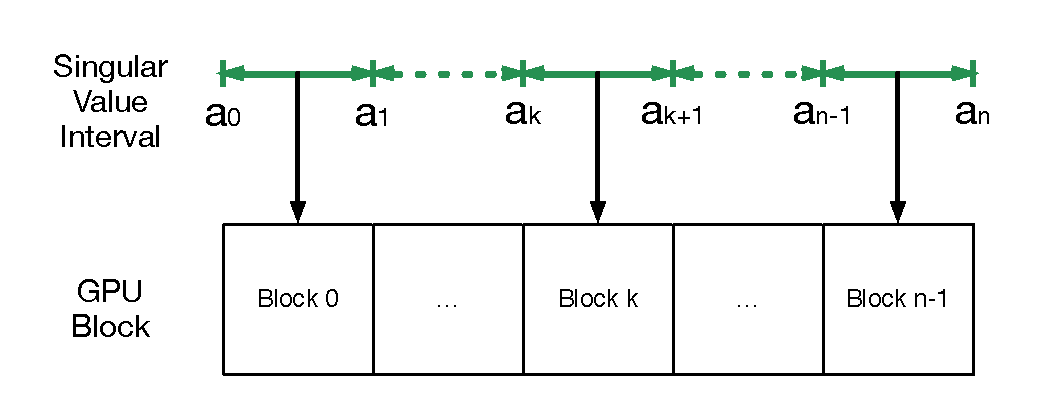
\includegraphics[width=0.5\textwidth]{length_interval}
  \label{fig:length_interval}
  }
  \subfigure[Equal Number Division]
  {
  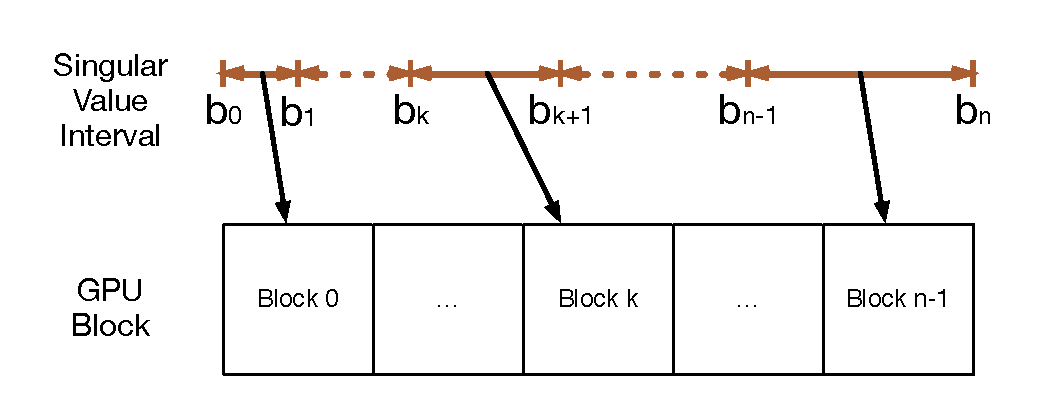
\includegraphics[width=0.5\textwidth]{number_interval}
  \label{fig:number_interval}
  }
  \caption{Division Strategies of interval}
\end{figure}
For the first step, we design the strategy to separate the interval by the length shown in Fig.\ref{fig:length_interval}.
In this strategy, we divide the whole interval $[a_0, a_n)$ into $n$ subintervals with the same length, while every subinterval may not have the same number of singular values usually.
In mathematical word, this strategy can be expressed as% $a_{k+1}-a_k = a_{k}-a_{k-1}$ and $NegCount(b_{k+1})-NegCount(b_{k}) \ne NegCount(b_{k})-NegCount(b_{k-1})$.
\begin{eqnarray}
a_{k+1}-a_k = a_{k}-a_{k-1} \hspace{2cm} \\
NegCount(a_{k+1})-NegCount(a_{k}) \ne \hspace{1cm} \nonumber\\
NegCount(a_{k})-NegCount(a_{k-1})
\end{eqnarray}

\begin{algorithm}
%\small
\caption{Equal Length Subinterval Algorithm}
\label{alg:lengthsub}
\begin{algorithmic}[1]
\Procedure{$\mathbf{Length\_Divide}$}{$n, B, t, \tau$}
  \State Obtain singular value boundary $[l,u)$ of matrix $B$;
  \State Define the thread ID $i$, $i<t$;
  \State Obtain average step $s = (u-l) / t $;
  \State Lower bound $\alpha = l + i * s$;
%  \State Upper bound $\beta = max(l + (i+1) * s, \alpha)$;
  \State $n_{\alpha} = NegCount(\alpha)$;
%  \State $n_{\beta} = NegCount(\beta)$;
%  \State $\alpha = \min(\alpha,\beta)$;
%  \State $\beta = \max(\alpha, \beta)$;
%  \State $n_{\alpha} = \min(n_{\alpha},n_{\beta})$;
%  \State $n_{\beta} = \max(n_{\alpha}, n_{\beta})$;
%  \State Max scan to refine $\alpha, \beta, n_{\alpha}, n_{\beta}$
%  \State Call $Bisection(val, n, B, \alpha, \beta, n_{\alpha}, n_{\beta}, \tau)$
  \State save the division point $\alpha$ and $n_{\alpha}$
\EndProcedure
\end{algorithmic}
\end{algorithm}

The parallel algorithm of length division working in GPU threads is shown in Algorithm \ref{alg:lengthsub}.
The length division strategy is easy to design.
However, it is not flexible to determine the number of subintervals for a better speedup.
This is because the determination of number of blocks is based on multiple aspects, such as the maximum number of threads, the number of threads in GPU warp, and the size of matrix.
The maximum number of threads per block determines the minimum number of blocks should be allocated.
The number in threads in GPU warp makes sure the suitable subintervals for best GPU utilization level.

Even we separate the interval with the best GPU utilization level, the speedup of length division cannot also reach a high level.
To achieve a even better speedup, we use another strategy to spearate the whole interval by the number of singular values in Fig.\ref{fig:number_interval}.
In this strategy, we divide the interval $[b_0,b_n)$ into $n$ subintervals with the same number of singular value.
However, the length of the subinterval may not be equal to others.
The mathematical representation can be writed as %$NegCount(b_{k+1})-NegCount(b_{k})=NegCount(b_{k})-NegCount(b_{k-1})$ but $b_{k+1}-b_k \ne b_{k}-b_{k-1}$
\begin{eqnarray}
b_{k+1}-b_k \ne b_{k}-b_{k-1} \hspace{2cm} \\
NegCount(b_{k+1})-NegCount(b_{k}) = \hspace{1cm} \nonumber\\
NegCount(b_{k})-NegCount(b_{k-1})
\end{eqnarray}
The parallel algorithm with same number of singular value is shown in Algorithm \ref{alg:numsub}.
\begin{algorithm}
%\small
\caption{Equal Number of Singular Value Subinterval Algorithm}
\label{alg:numsub}
\begin{algorithmic}[1]
\Procedure{$\mathbf{Number\_Divide}$}{$n, B, t, \tau$}
  \State Obtain singular value boundary $[l,u)$ of matrix $B$;
  \State Define the thread ID $i$, $i<t$;
  \State $mid = inside(l, u, B)$;
  \State $n_m = NegCount(n, B, mid)$;
  \While {$n_m \ne (i+1)n/t$ and $mid-l > \tau$}
    \If {$n_m \ge (i+1)n/t$}
      \State $u=mid$;
      \State $n_u=n_m$;
    \Else
      \State $l=mid$;
      \State $n_l=n_m$;
    \EndIf
    \State $mid = inside(l, u, B)$;
    \State $n_m = NegCount(n, B, mid)$;
  \EndWhile
  \State save the division point $mid$ and $n_m$.
\EndProcedure
\end{algorithmic}
\end{algorithm}


We calculate the boundary points of the subintervals from the first step based on Algorithm \ref{alg:lengthsub} and Algorithm \ref{alg:numsub}. 
Either algorithm works in one block with multiple threads.
Every thread is responsible for one spliting point.
The second step is to calculate the exact singular values in these subintervals with Algorithm \ref{alg:bisection}.

In our design, one subinterval is allocated into one GPU block.
In other words, one GPU block will calculate all the singular values in its corresponding subinterval.
%Suppose the whole interval can be divided into $N$ subintervals, every block processes one subintervals, and thus $N$ blocks are needed.
Inside the block, multiple threads are working concurrently.
One thread will obtain one singular value in the subinterval.
%Suppose the number of singular values in one block is $M$, thus $M$ is the number of threads in the block.

\subsection{Singular Vector Kernel}
The singular vector kernel is designed based on Algorithm \ref{alg:twisted}.
First, we achieve the algorithm without any optimization.
But the 10X speedup compared to CPU is low because of the heavy usage of global memory and the low global memory throughput.
After we utilize the local memory and shared memory instead of frequent-used global memory and change the matrix arrangement from row-major to column-major.
The performance nearly doubled.

Since the singular vectors are two $n\times n$ matrices, the memory on GPU will effect the maximum matrix size.
Based on our desing, all the singular vectors require $5\times n^2$ floating numbers.
Thus, the maximum matrix size is determined by
\begin{equation}
m_t = \sqrt{U / (5 * 4)}
\label{eq:max_size}
\end{equation}
where $U$ is the memory size of GPU, $4$ means the size of float number.

\subsection{Huge Size Solution}
In our design, the maximum singular values can be processed on a singular GPU is $m_b = block\_size \times thread\_block\_size$,
while the maximum singular vectors are determined by Equation \ref{eq:max_size}.
Usually, $m_b$ is much larger than $m_t$.
For Tesla K40c with 16GB memory, $m_t = 24K$, while $m_b = 262K$
However, when the matrix size becomes larger than $m_t$, even larger than $m_b$,
the singular vector kernel cannot obtain all singular vectors at the same time.
In this subsection, we introduce a divide-and-conquer architecture to solve the huge matrix size.

When matrix size is less than $m_b$, but larger than $m_t$ from Equation \ref{eq:max_size},
we only need to separate the singular vectors into small pieces which can be processed by a single GPU.
When matrix size is larger than $m_b$, we should separate both singular values and singular vectors into small pieces.

The division of singular value can be divided by $m_b$ directly.
Thus, there are $l_b = \lfloor(n/m_b)\rfloor + 1$ pieces, and each pieces has $\lfloor(n/l_b)\rfloor$ singular values.

The division of singular vector should take memory size into consider.
The maximum pieces $l_t$ can be rewrite from Equation \ref{eq:max_size} as follow:
\begin{equation}
l_t = \sqrt{U/(5 * n * 4)}
\label{eq:max_length}
\end{equation}
where $n$ is matrix size.
Thus, There should be $\lfloor(n/l_t)\rfloor+1$ pieces with $\lfloor(n/l_t)\rfloor$ singular vectors each pieces.
For a single GPU, the execution between every pieces is serial.
When one piece finished, GPU processes the next one, until the last one.
Thus, the execution time is the summation of every subsection.
Equation \ref{eq:max_length} also provides the theorical maximum matrix size can be processed on GPUs when set $l=1$.
For Tesla K40c, the theorical maximum matrix size is $600$ million.
However, the singular vector kernel will not have speedup compared to execution on CPU.

When matrix size is huge, only one GPU is not enough to speed up the SVD.
We make use of pthread to control mutiple GPUs.
Each thread created by pthread takes control of one GPU.

We also build a two-computer network to speed up the SVD.
In our design, each computer has one GPU and communicated through sockets.



\section{Experiment Result}
In this section, we will analyze the performance of our algorithm compared to other SVD implementations on CPU and GPU.
In addition, we will discuss the GPU kernel profiling result to show how to improve our implementations.
We also show our performance on huge matrix size.

We tested our algorithm on GeForce 750 Ti, Quadro 600 and Tesla K40c.
The specifications are in Table \ref{tab:spec}.
\begin{table}[h]
\caption{Specifications of Different GPUs}
\centering
\begin{tabular}{|c|c|c|c|}
\hline
Specifications & GeForce 750 & Quandro 600 & Tesla K40 \\ \hline
Architecture   &     Maxwell &       Fermi &    Kepler \\ \hline
CUDA Cores     &         640 &          96 &      2880 \\ \hline
GPU Clock      &    1268 MHz &    1280 MHz &   745 MHz \\ \hline
Mem Size       &        2 GB &        1 GB &     12 GB \\ \hline
Mem Bandwidth  &   86.4 GB/s &   25.6 GB/s &  288 GB/s \\ \hline
\end{tabular}
\label{tab:spec}
\end{table}

\subsection{Comparision to other implementations}
We generated random bidiagonal matrices with double precision numbers in the range of 0 to 1.
In order to obtain relative accuracy experimental results, we generates 10 random matrices.
For each matrix, the SVD algorithm was executed 10 times on GPU.
The average performance does not vary much when more matrices and more times are used.

We compare our algorithm with CULA GPU library, Intel MKL library, Sheetal's QR implementation on S1070, and Liu's divide-and-conquer implementation on M2070.
We measure the performance of CULA on Tesla K40c, and that of Intel MKL on an 8-core cpu with 16 threads.
Until now, CULA library only has QR routine culaDbdsqr.
Intel MKL library has both divide-and-conquer DBDSDC and QR routine DBDSQR.
Usually, divide-and-conquer routine is faster than QR routine, so we select DBDSDC instead of DBDSQR.
We measure the performance of CULA on Tesla K40c, and that of Intel MKL on an 8-core cpu with 16 threads.
For Sheetal's implementation, we use the experimental results of diagonalization listed in the table of their papers.
The results of Liu's are estimated comprehensively according to the figures presented in their paper.

\begin{figure}[hbpt]
\centering
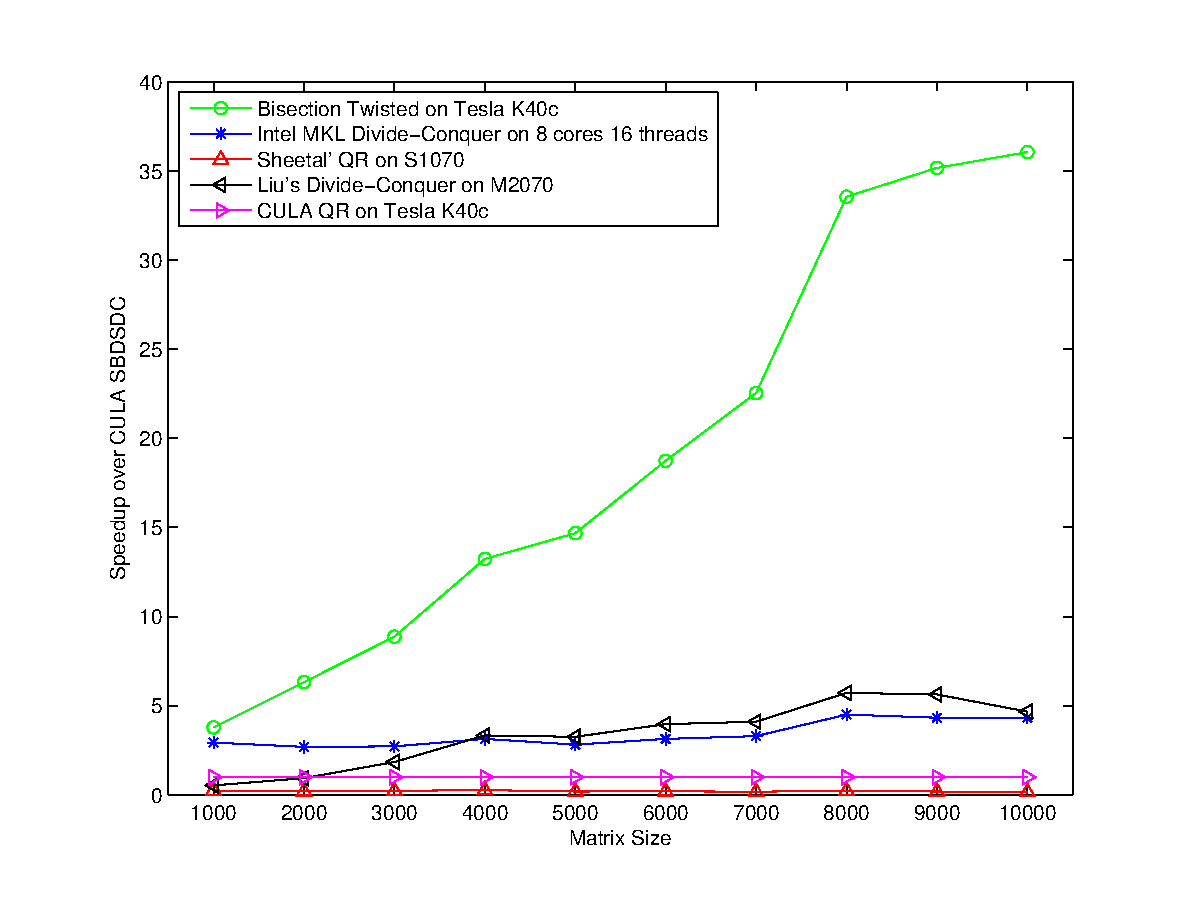
\includegraphics[width=0.5\textwidth]{svd_speedup}
\caption{Overall Performance Comparision}
\label{fig:svd_speedup}
\end{figure}
Figure \ref{fig:svd_speedup} shows the performance of our implementation on Tesla K40c GPU to other existing libraries and implementations.
We selects CULA QR routine BDBSQR as a baseline.
From the figure, we achieve a speedup of 3.8 to 36 over CULA culaDbdsqr routine,
while Intel MKL DBDSDC routine has a 2.9 to 4.3 speedup on a 8 core cpu, and Liu's implementation has only 0.5 to 4.7 speedup over CULA library.
Sheetal's implementation is about 3 to 5.3 times slower than CULA library.
The performance goes up when matrix size becomes large.
Overall, we achieve a speedup of 1.3 to 8.3 over the Intel MKL Divide-Conquer Implementation on CPU, 4 to 7.2 over the Liu's Divide-conquer method, 15 to 288 over the QR implementation Sheetal Paper.

\subsection{Profiling Data}

\subsubsection{the Optimal Block Size}
In our length division design on singular value, the number of block size determines the execution time of the whole singular values.
An inappropriate block division will affect the performance on GPU heavily.
To obtain the optimal block size, we make use of experimental method. 

\begin{figure}[hbpt]
\centering
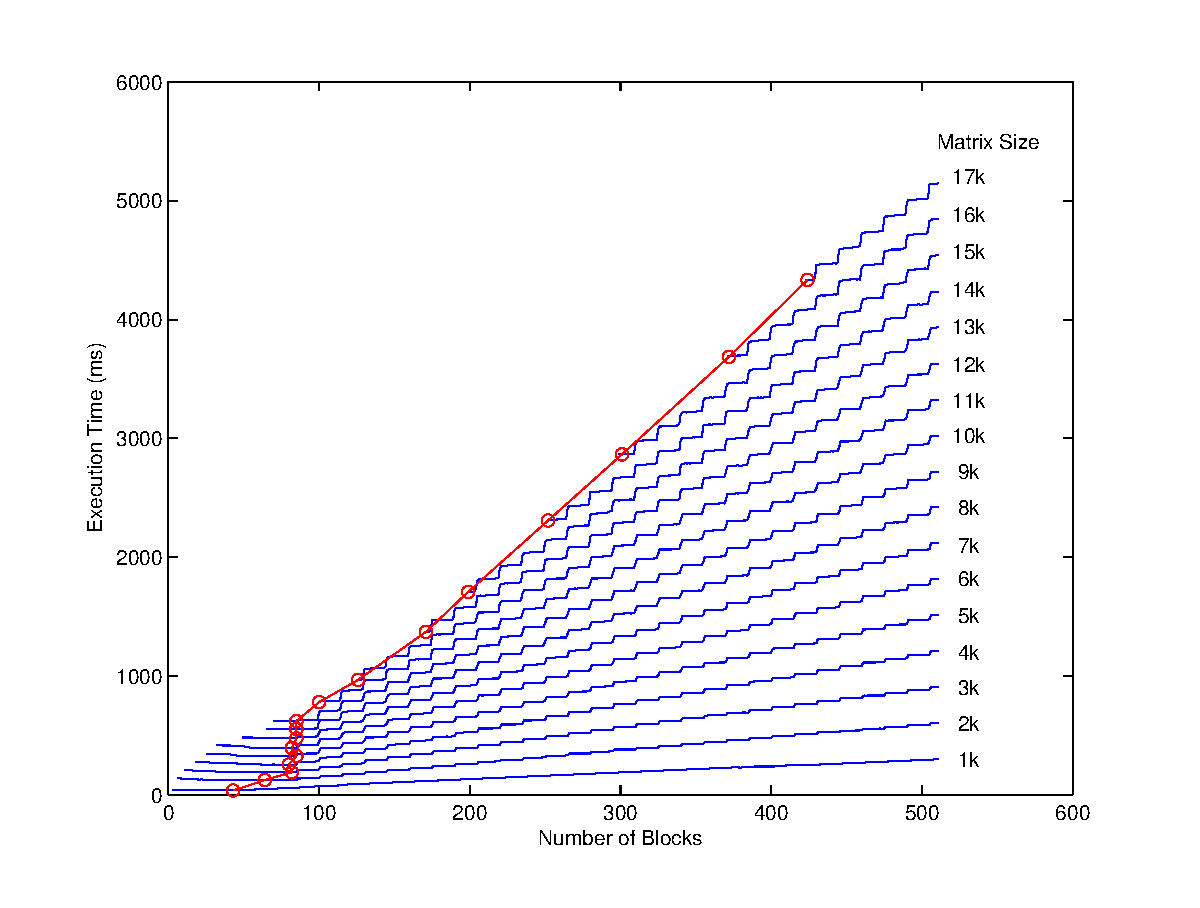
\includegraphics[width=0.5\textwidth]{length_block_num}
\caption{The optimal block number of different matrix size with double precision on Tesla K40c}
\label{fig:length_block_num}
\end{figure}
Figure \ref{fig:length_block_num} shows the elasped time of obtaining all the singular values with different number of blocks and different matrix size on GPU Tesla K40c with double precision.
The blue wavy curves show the relationship between the execution time and the number of blocks on the matrix size in the right column.
From the curves, we can see that the performance goes down slightly first, and then rises when the number of blocks increases.
The left point of the wavy curve shows the minimal number of blocks should be allocated when the matrix size is identified.
In other words, the number of blocks should not be less than the left point on the wavy curves.
When matrix size becomes large, the left point in wave curve trends to a large number of blocks.

The red circle curve in the figure shows the optimal number of blocks with minimal execution time on different size.
we can see that the optimal number of blocks increases when matrix size is less than $3k$,
keeps stable when matrix size is in the range of $3k$ to $9k$,
and becomes the minimal number of blocks when matrix size is lager than $9K$.
Actually, when the block number is close to the optimal number, the execution time does not change too much.
Due to the uncertainty of the input matrix, the optimal block number may vary slightly.
Thus, it is not necessary to select the exact optimal block number.
But it is better to select the number of blocks around the optimal one.

\begin{figure}[hbpt]
\centering
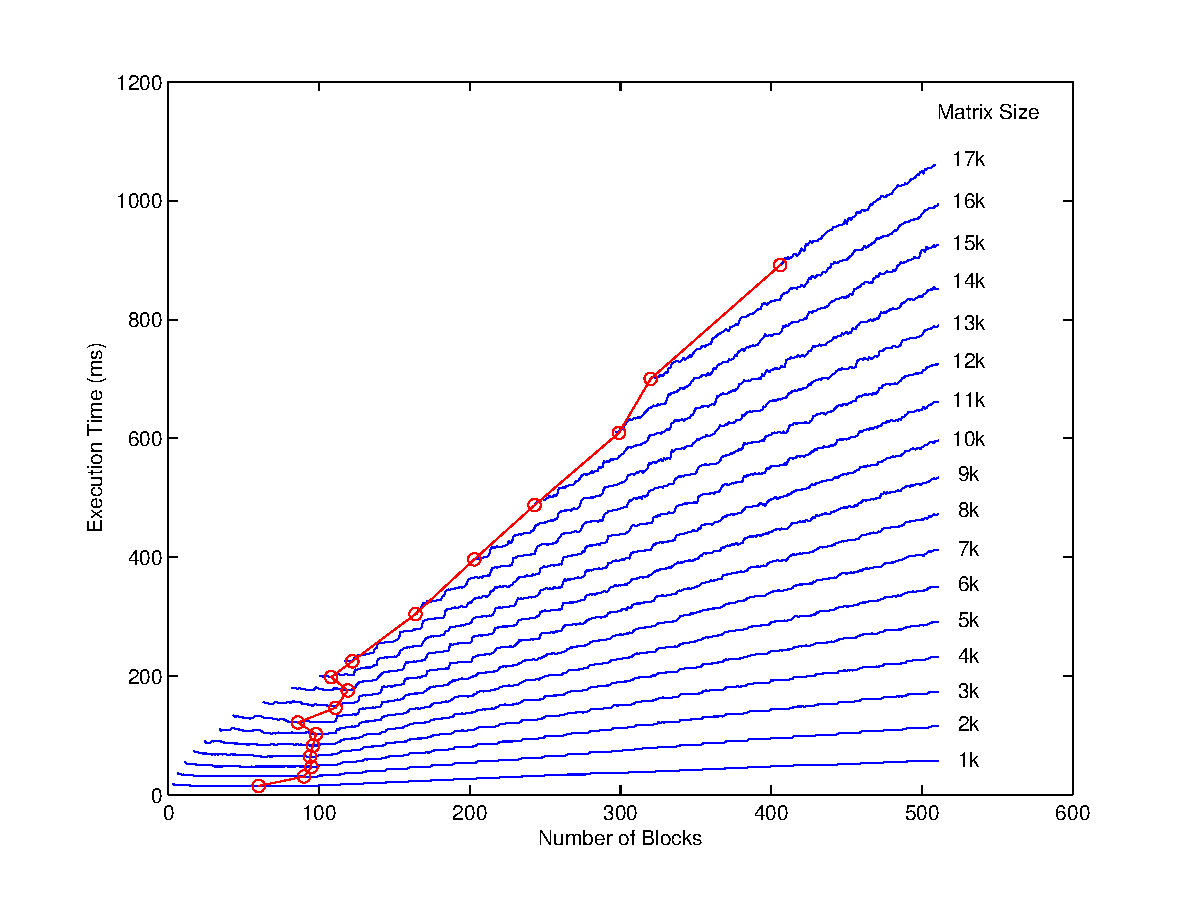
\includegraphics[width=0.5\textwidth]{length_block_single}
\caption{The optimal block number of different matrix size with single precision on GeForce 750 Ti}
\label{fig:length_block_single}
\end{figure}
Figure \ref{fig:length_block_single} is another experimental results on GeForce 750 Ti GPU with single precision.
The curves are very similar with the curves in Figure \ref{fig:length_block_num}.
However, the optimal number of blocks shifts right to be a large number because GeForce has a better architecture than Tesla.
%The reason of the optimal number of blocks is determined by the CUDA cores.
%The Tesla K40c has 15 multiprocessors (MP) and 192 CUDA cores per MP.
%Thus, the total CUDA cores are $2880$ in Tesla K40.
%The GPU code is actually executed in groups of 32 threads called a warp concurrently.

%The optimal GPU block size is not the less, the better.
%It depends on the number of singular values in the subintervals.
%If one have more, GPU will have to wait.
%If all subintervals have the number of singular deviate from the integer multiples of a warp. The GPU efficiency will be less.

\subsubsection{Comparasion of two different Singular Value Design}
In this part, we compare the execution time on two different singular value kernels.
For the length division design, we selects the minimal execution time corresponding to red point curve in figure \ref{fig:length_block_num}.
For the number division design, we selects the minimal number of blocks that is able to allocated, since the execution time does not vary much between the minimal number of blocks and the optimal nubmer of blocks.

\begin{figure}[hbpt]
\centering
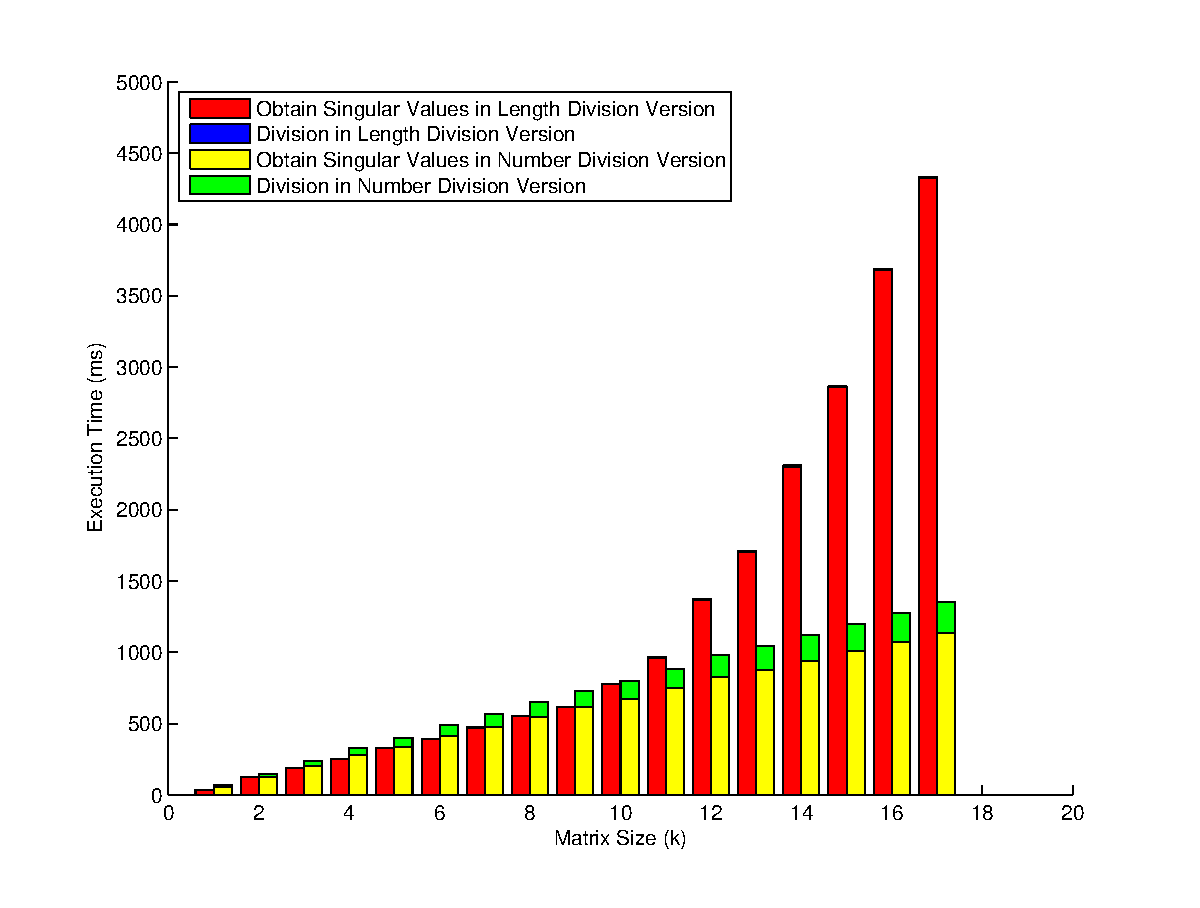
\includegraphics[width=0.5\textwidth]{compare_value_kernel}
\caption{The optimal block number of different matrix size with single precision on GeForce 750 Ti}
\label{fig:compare_value_kernel}
\end{figure}
Figure \ref{fig:compare_value_kernel} shows the execution time of obtaining all singular values of two different implementations on GPU.
The left bar is the execution time of length division design, while the right bar is that of number division design.
From the figure, we can see that when matrix size is less than $9k$, length division version run a little faster than number division version.
When matrix size is larger than $9k$, the execution time of length division version rises quickly, while the execution time of number division version only rises linearly.
Thus, when matrix size becomes larger than $9k$, it is better to select number division kernel.

Also, figure \ref{fig:compare_value_kernel} represents the average execution time on each GPU kernels of two different designs.
When matrix size is smaller than $9k$, the difference between two designs is only on the interval division method.
The division time in length division version is negligible since it is two small, while the division time in number division version increases.
The execution time on obtaining singular values in both version are almost the same when matrix size is less than $9k$.

\subsubsection{Profiling Analysis on Different GPUs}
\textbf{I want to analyze the bound}

\begin{figure}[hbpt]
\centering
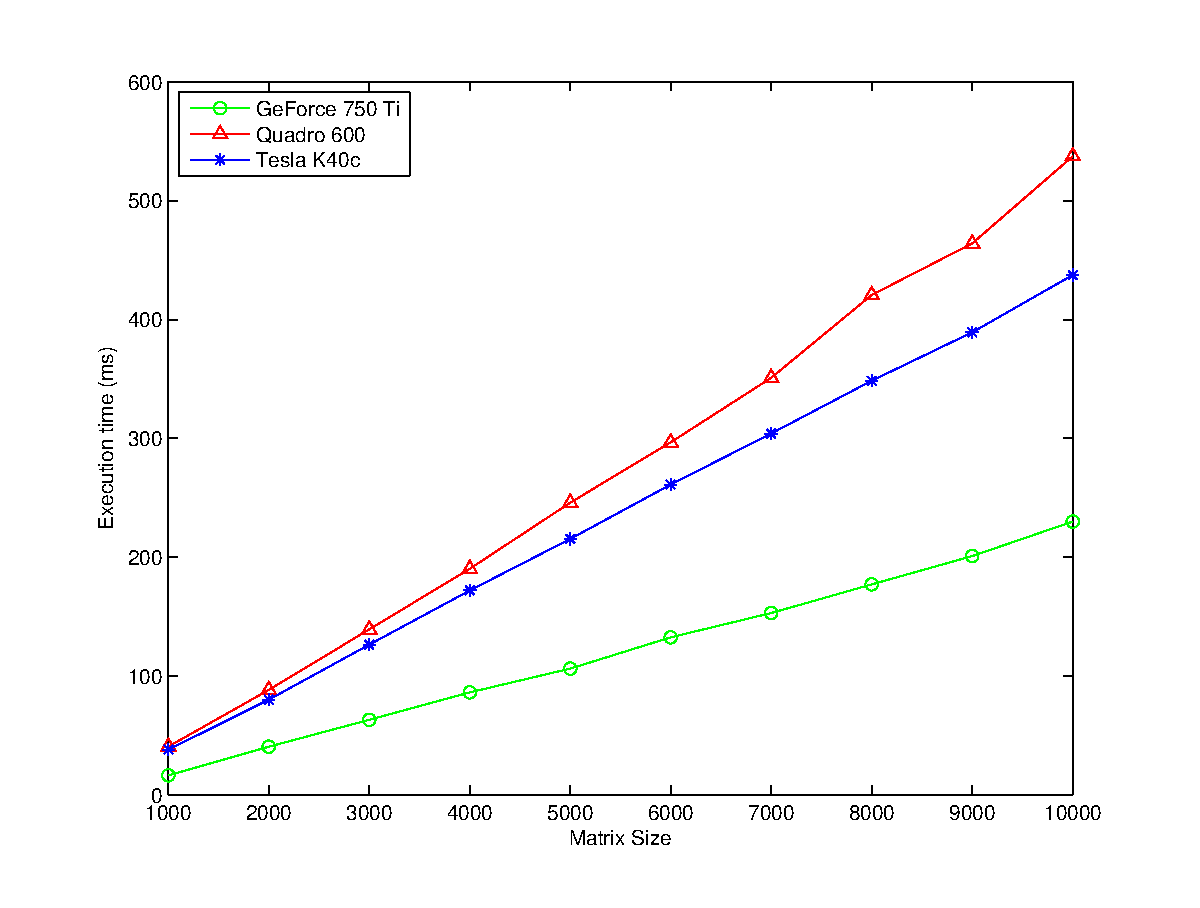
\includegraphics[width=0.5\textwidth]{svd_val_gpus}
\caption{Execution time of number-division singular value kernel on different GPUs with single-float precision}
\label{fig:svd_val}
\end{figure}
Figure \ref{fig:svd_val} shows the execution time of singular value kernel on different GPUs. 

\begin{figure}[hbpt]
\centering
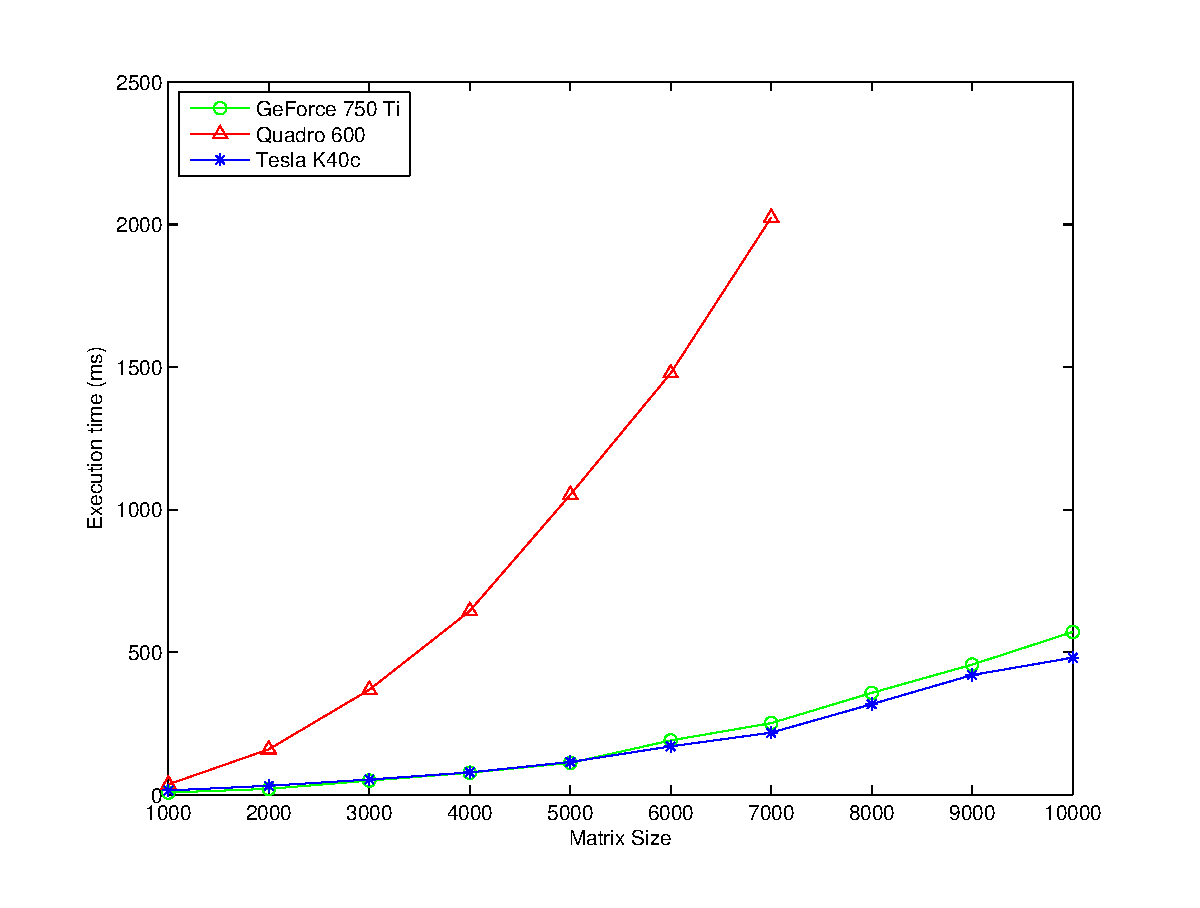
\includegraphics[width=0.5\textwidth]{svd_vec_gpus}
\caption{Execution time of singular value kernel on different GPUs with single-float precision}
\label{fig:svd_vec}
\end{figure}
Figure \ref{fig:svd_vec} shows the execution time of singular vector kernel on different GPUs. 

\subsubsection{Tolerance in Bisection Algorithm}
Since the bisection algorithm is an approximate algorithm to calculate the singular values, we should test the effect of different error tolerance.
The error tolerance $err$ means that the error between the singular values of our algorithm and the actual singular values are less than $err$.
It determines the accuracy of singular value and therefore the orthogonality of singular vectors.
As we know, the more accuracy of singular values are, the more execution time should be spent.
However, it is important to know the incremental execution time to determine which error tolerance is suitable for different applications.
We test our algorithm on different error tolerance.
The error tolerance is between $10^{-5}$ to $10^{-16}$ with tenfolder decreasing.

\textbf{I'm still thinking how to draw this figure.}
\begin{figure}[hbpt]
\centering
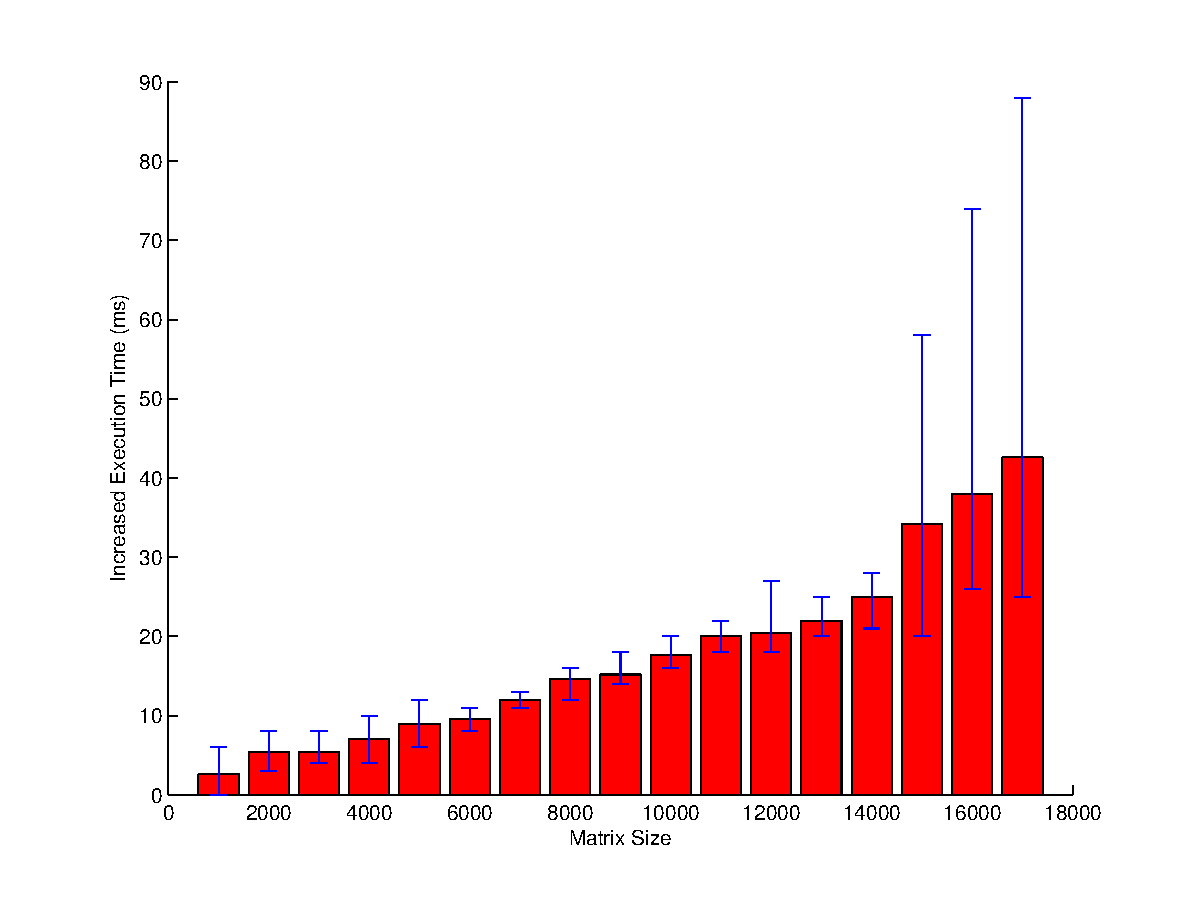
\includegraphics[width=0.5\textwidth]{tolerance}
\caption{Average Extra Execution Time When the accuracy increase Performance Comparision}
\label{fig:tolerance}
\end{figure}
Figure \ref{fig:tolerance} shows the average increased execution time when the accuracy of singular values goes up a higher level on different matrix size.
In other word, it shows the average increased execution time when the error tolerance becomes smaller from $10^{-x}$ to $10^{-(x+1)}$.
From the figure, we can see that when matrix size is smaller than 12000, the additional execution time is only less than $20 ms$ when the error tolerance rises a level.
When the matrix size is larger than 15000, the additional execution time is a little higher about $40 ms$ per level.

\subsection{Pthread CUDA Result}
\subsubsection{Load Balance}
\begin{figure}[hbpt]
\centering
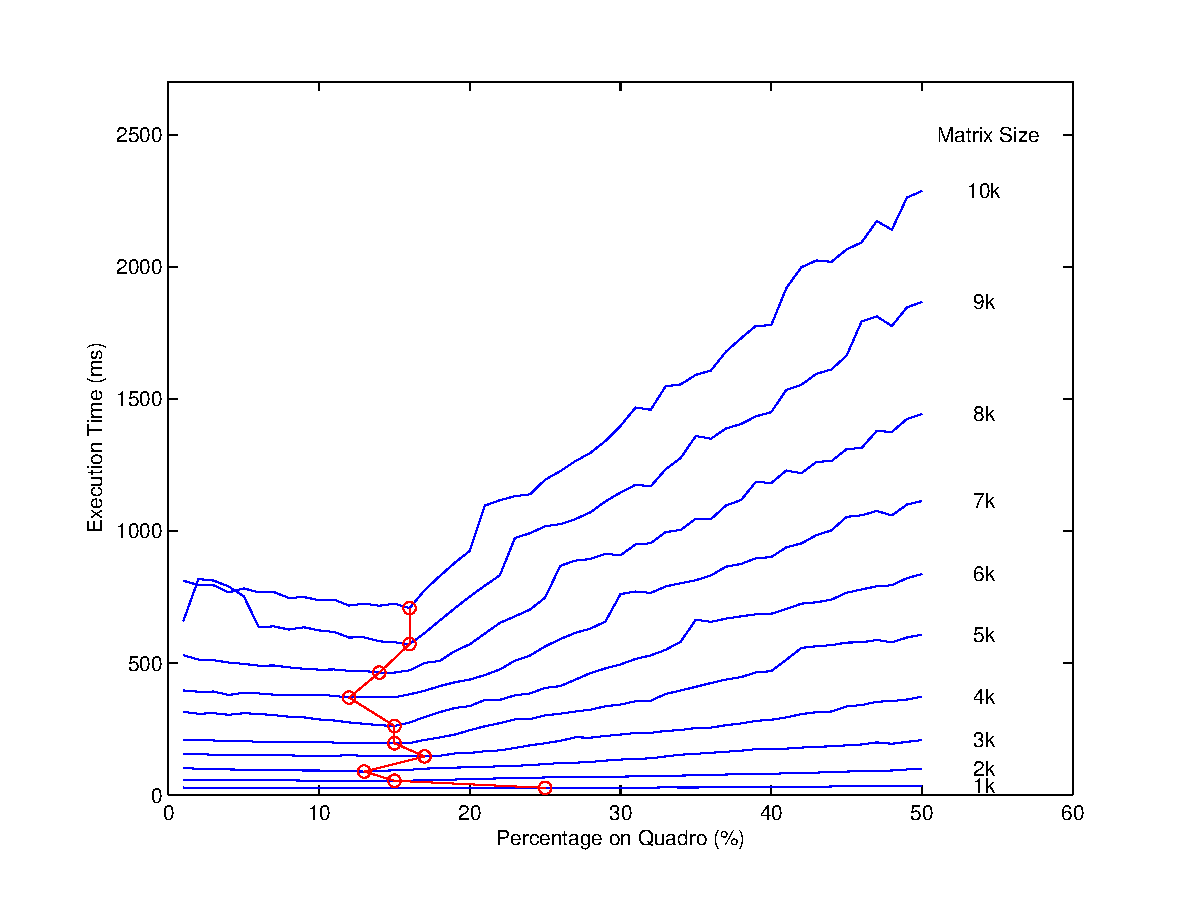
\includegraphics[width=0.5\textwidth]{pthread}
\caption{Load Balance on GeForce and Quadro}
\label{fig:pthread}
\end{figure}
Figure \ref{fig:pthread} shows the total execution time with different load balance on a system of two different GPUs.
The horizontal axis represents the percentage of work on Quadro 600.
The other percentage of work will be moved to GeForce 750 Ti obviously.
The red points represent the minimum values in the blue curves.
The blue curves can be separated into two parts by red points.
The left ones are dominated by GeForce 750 Ti, while the right ones are contributed by Quadro 600.
Since Quadro 600 has a worse performance than GeForce 750 Ti, less work is allocated on it.
When around 15\% of work is executed on Quadro 600, and 85\% of that is processed on GeForce 750 Ti,
the total performance of the system will be better than others.

\textbf{A table to shows the Huge Size Result. This part do not compare to other results.} 

\begin{table}[h]
\caption{Performance of Huge Size Matrix}
\centering
\begin{tabular}{|c|c|c|c|c|c|c|}
\hline
Matrix & \multicolumn{6}{|c|}{Number of GPUs} \\ \cline{2-7}
Size & 1 & 2 & 3 & 4 & 5 & 6 \\ \hline
100K   &   442s  &   224s  &   159s  &   123s  &    98s  &    87s\\ \hline
200K   &  1666s  &   837s  &   564s  &   427s  &   341s  &   291s\\ \hline
500K   & 13007s  &  6516s  &  4355s  &  3280s  &  2626s  &  2191s\\ \hline
1000K  & 64591s  & 32333s  & 21597s  & 16219s  & 12983s  & 10836s\\ \hline
\end{tabular}
\label{tab:hresult}
\end{table}



\section{conclusion}



% An example of a floating figure using the graphicx package.
% Note that \label must occur AFTER (or within) \caption.
% For figures, \caption should occur after the \includegraphics.
% Note that IEEEtran v1.7 and later has special internal code that
% is designed to preserve the operation of \label within \caption
% even when the captionsoff option is in effect. However, because
% of issues like this, it may be the safest practice to put all your
% \label just after \caption rather than within \caption{}.
%
% Reminder: the "draftcls" or "draftclsnofoot", not "draft", class
% option should be used if it is desired that the figures are to be
% displayed while in draft mode.
%
%\begin{figure}[!t]
%\centering
%\includegraphics[width=2.5in]{myfigure}
% where an .eps filename suffix will be assumed under latex, 
% and a .pdf suffix will be assumed for pdflatex; or what has been declared
% via \DeclareGraphicsExtensions.
%\caption{Simulation Results}
%\label{fig_sim}
%\end{figure}

% Note that IEEE typically puts floats only at the top, even when this
% results in a large percentage of a column being occupied by floats.


% An example of a double column floating figure using two subfigures.
% (The subfig.sty package must be loaded for this to work.)
% The subfigure \label commands are set within each subfloat command, the
% \label for the overall figure must come after \caption.
% \hfil must be used as a separator to get equal spacing.
% The subfigure.sty package works much the same way, except \subfigure is
% used instead of \subfloat.
%
%\begin{figure*}[!t]
%\centerline{\subfloat[Case I]\includegraphics[width=2.5in]{subfigcase1}%
%\label{fig_first_case}}
%\hfil
%\subfloat[Case II]{\includegraphics[width=2.5in]{subfigcase2}%
%\label{fig_second_case}}}
%\caption{Simulation results}
%\label{fig_sim}
%\end{figure*}
%
% Note that often IEEE papers with subfigures do not employ subfigure
% captions (using the optional argument to \subfloat), but instead will
% reference/describe all of them (a), (b), etc., within the main caption.


% An example of a floating table. Note that, for IEEE style tables, the 
% \caption command should come BEFORE the table. Table text will default to
% \footnotesize as IEEE normally uses this smaller font for tables.
% The \label must come after \caption as always.
%
%\begin{table}[!t]
%% increase table row spacing, adjust to taste
%\renewcommand{\arraystretch}{1.3}
% if using array.sty, it might be a good idea to tweak the value of
% \extrarowheight as needed to properly center the text within the cells
%\caption{An Example of a Table}
%\label{table_example}
%\centering
%% Some packages, such as MDW tools, offer better commands for making tables
%% than the plain LaTeX2e tabular which is used here.
%\begin{tabular}{|c||c|}
%\hline
%One & Two\\
%\hline
%Three & Four\\
%\hline
%\end{tabular}
%\end{table}


% Note that IEEE does not put floats in the very first column - or typically
% anywhere on the first page for that matter. Also, in-text middle ("here")
% positioning is not used. Most IEEE journals/conferences use top floats
% exclusively. Note that, LaTeX2e, unlike IEEE journals/conferences, places
% footnotes above bottom floats. This can be corrected via the \fnbelowfloat
% command of the stfloats package.




% conference papers do not normally have an appendix


% use section* for acknowledgement
\section*{Acknowledgment}


The authors would like to thank...
more thanks here


% trigger a \newpage just before the given reference
% number - used to balance the columns on the last page
% adjust value as needed - may need to be readjusted if
% the document is modified later
%\IEEEtriggeratref{8}
% The "triggered" command can be changed if desired:
%\IEEEtriggercmd{\enlargethispage{-5in}}

% references section

% can use a bibliography generated by BibTeX as a .bbl file
% BibTeX documentation can be easily obtained at:
% http://www.ctan.org/tex-archive/biblio/bibtex/contrib/doc/
% The IEEEtran BibTeX style support page is at:
% http://www.michaelshell.org/tex/ieeetran/bibtex/
%\bibliographystyle{IEEEtran}
% argument is your BibTeX string definitions and bibliography database(s)
%\bibliography{IEEEabrv,../bib/paper}
%
% <OR> manually copy in the resultant .bbl file
% set second argument of \begin to the number of references
% (used to reserve space for the reference number labels box)

\begin{thebibliography}{1}

\bibitem{97bookalgebra}
James W. Demmel,
\emph{Applied Numerical Linear Algebra}, 1st~ed.
\hskip 1em plus 0.5em minus 0.4em\relax
Philadelphia, USA: Society for Industrial and Applied Mathematics, 1995.

\bibitem{95ETNAbisecion}
James W. Demmel, Inderjit Dhillon, and Huan Ren.
\emph{ON THE CORRECTNESS OF SOME BISECTION-LIKE PARALLEL EIGENVALUE ALGORITHMS IN FLOATING POINT ARITHMETIC}
\hskip 1em plus 0.5em minus 0.4em\relax
Electronic Transactions on Numerical Analysis. Volume 3, pp. 116-149, December 1995.

\bibitem{65SIAM}
G. Golub and W. Kahan
\emph{Calculating the Singular Values and Pseudo-Inverse of a Matrix},
\hskip 1em plus 0.5em minus 0.4em\relax
SIAM Journal for Numerical Analysis; Vol. 2, \#2; 1965

\bibitem{06bookhandbook}
Leslie Hogben, Kenneth H Rosen.
\emph{Handbook of Linear Algebra}.
\hskip 1em plus 0.5em minus 0.4em\relax
Taylor \& Francis Group, LLC, 2007.

\bibitem{09NLAAtwisted}
W. Xu, S. Qiao,
\emph{A twisted factorization method for symmetric SVD of a complex symmetric tridiagonal matrix},
\hskip 1em plus 0.5em minus 0.4em\relax
Numerical Linear Algebra with Applications, 16 (10) (2009), pp. 801–815

\bibitem{05UCB}
P.R. Willems, B. Lang, and C. V\"{o}mel,
\emph{LAPACK WORKING NOTE 166: COMPUTING THE BIDIAGONAL SVD USING MULTIPLE RELATIVELY ROBUST REPRESENTATIONS}
\hskip 1em plus 0.5em minus 0.4em\relax
EECS Department, University of California, Berkeley, Tech. Rep. UCB/CSD-05-1376, 2005.

\bibitem{09IPDPSQR}
Sheetal Lahabar, P. J. Narayanan,
\emph{Singular Value Decomposition on GPU using CUDA},
\hskip 1em plus 0.5em minus 0.4em\relax
Proc. IEEE Int',l Symp. Parallel and Distributed Processing, pp. 1-10, 2009.

%\bibitem{11IPDPSQR}
%M. Anderson, G. Ballard, J. Demmel, and K. Keutzer,
%\emph{Communication-avoiding QR decomposition for GPU}
%\hskip 1em plus 0.5em minus 0.4em\relax
%Proc. IEEE Int',l Symp. Parallel and Distributed Processing, pp. 48-58, 2011.

\bibitem{13CFDC}
Ding Liu, Ruixuan Li, David J. Lilja and Weijun Xiao
\emph{A divide-and-conquer approach for solving singular value decomposition on a heterogeneous system}
\hskip 1em plus 0.5em minus 0.4em\relax
CF'13 Proceedings of the ACM International Conference on Computing Frontiers Article No. 36 

\bibitem{14arxivjacobi}
Vedran Novakovic,
\emph{A hierarchically blocked Jacobi SVD algorithm for single and multiple graphics processing units},
\hskip 1em plus 0.5em minus 0.4em\relax
\url{http://arxiv.org/abs/1401.2720v2}

\bibitem{cublas}
\emph{NVIDIA CUDA CUBLAS library}, 2nd~ed, NVIDIA Corporation (August 2010)

\bibitem{cula}
John R. Humphrey, Daniel K. Price, Kyle E. Spagnoli, Aaron L. Paolini and Eric J. Kelmelis
\emph{CULA: hybrid GPU accelerated linear algebra routines},
\hskip 1em plus 0.5em minus 0.4em\relax
Proc. SPIE 7705, Modeling and Simulation for Defense Systems and Applications V, 770502 (April 26, 2010); doi:10.1117/12.850538;
\url{http://dx.doi.org/10.1117/12.850538}

\bibitem{magma}
Agullo, E., Demmel, J., Dongarra, J., Hadri, B., Kurzak, J., Langou, J., Ltaief, H., Luszczek, P., Tomov, S.
\emph{Numerical linear algebra on emerging architectures: The PLASMA and MAGMA projects},
\hskip 1em plus 0.5em minus 0.4em\relax
Journal of Physics: Conference Series, Vol. 180, 2009.

\bibitem{58iter1}
M. R. Hestenes,
\emph{Inversion of matrices by biorthonalization and related results},
\hskip 1em plus 0.5em minus 0.4em\relax
J. Soc. Indust. Appl. Math., 6 (1958), pp. 51–90.

\bibitem{90iter2}
J. Demmel and W. Kahan.
\emph{Accurate singular values of bidiagonal matrices}.
\hskip 1em plus 0.5em minus 0.4em\relax
SIAM J. Sci. Stat. Comput., 11(5):873-912, 1990.

\bibitem{65iter3}
G. Golub and W. Kanhan.
\item{Calculating the singular values and pseudo-inverse of a matrix}.
\hskip 1em plus 0.5em minus 0.4em\relax
SIAM J. Num. Anal. (Series B), 1965.

\bibitem{94DCSVD}
M. Gu, J. Demmel and I. Dhillon,
\emph{Efficient Computation of the Singular Value Decomposition with Applications to Least Squares Problems.}
\hskip 1em plus 0.5em minus 0.4em\relax
In Technical Report CS-94-257, Department of Computer Science, University of Tennessee,October 1994.

\end{thebibliography}




% that's all folks
\end{document}


